\frame{\titlepage}

%% Introduction
\frame{ \frametitle{Introduction}
  \begin{definition}[Binomial]
    Let $X$ represent the number of successes in a sequence of $n$ independent Bernoulli trials with probability of success $p$ on each trial.

    \vspace{3mm}
    \uncover<2->{
      $X$ has discrete pdf
      \begin{equation*}
        f_X(x) = \binom{n}{x} \; p^x q^{n-x}
      \end{equation*}
    }
    \uncover<3->{
      and cdf
      \begin{equation*}
        F_X(x) = P(X \leq x) = \sum_{k=0}^x f_X(k).
      \end{equation*}
    }
  \end{definition}
}
\frame{ \frametitle{Introduction}
  The binomial cdf is easy to calculate for small $n$ ...
  \pause

  But as $n$ gets larger, it becomes increasingly difficult.
  \pause

  For example ...
}
\frame{ \frametitle{Introduction}
  When $n=3$,
  \begin{equation*}
    F(1) = \binom{3}{1} \; p^1 q^2 + \binom{3}{0} \; p^0 q^3
  \end{equation*}
  \pause
  When $n=25$,
  \begin{align*}
    F(12) =& \binom{25}{12} \; p^{12} q^{13} + \binom{25}{11} \; p^{11} q^{14} + \binom{25}{10} \; p^{10} q^{15} + \binom{25}{9} \; p^9 q^{16} \\
          +& \binom{25}{8} \; p^8 q^{17} + \binom{25}{7} \; p^7 q^{18} + \binom{25}{6} \; p^6 q^{19} + \binom{25}{5} \; p^5 q^{20} \\
          +& \binom{25}{4} \; p^4 q^{21} + \binom{25}{3} \; p^3 q^{22} + \binom{25}{2} \; p^2 q^{23} + \binom{25}{1} \; p^1 q^{24} \\
          +& \binom{25}{0} \; p^0 q^{25}
  \end{align*}
}
\frame{ \frametitle{Introduction}
  A common technique is to use the normal distribution as an approximation:
  \begin{equation*}
    F_X(x) \approx \Phi \left( \frac{x + 0.5 - \mu}{\sigma} \right),
  \end{equation*}
  where $\mu = np$, $\sigma = \sqrt{np(1-p)}$, and $\Phi$ is the standard
  normal cdf.

  \pause
  \vspace{3mm}
  When does this work well? ... \pause In a nutshell, when the binomial is symmetric.
}
\frame{ \frametitle{Introduction}
  The binomial is symmetric when
  \uncover<1->{$p=0.5$}
  \uncover<2>{or $n$ is very large.}
  \begin{center}
    \only<1>{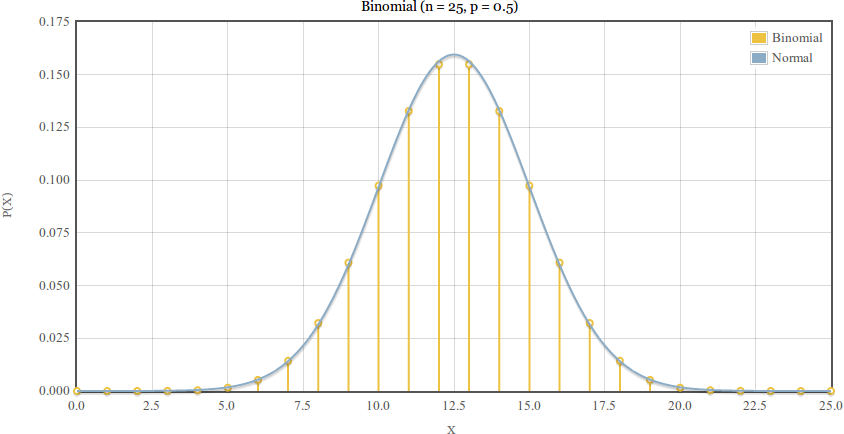
\includegraphics[width=\textwidth]{../images/binomial-normal-1.png}}
    \only<2>{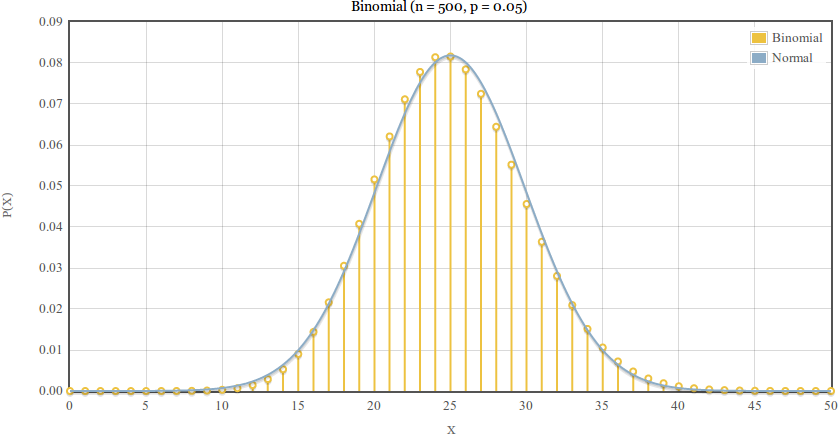
\includegraphics[width=\textwidth]{../images/binomial-normal-2.png}}
  \end{center}
}
\frame{ \frametitle{Introduction}
  However, when $n$ is medium and $p$ is extreme ...
  \begin{center}
    \only<1>{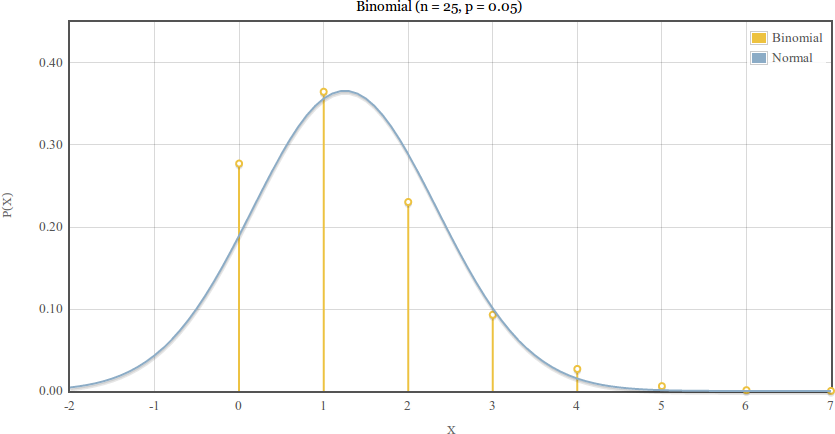
\includegraphics[width=\textwidth]{../images/binomial-normal-sn-1.png}}
    \only<2>{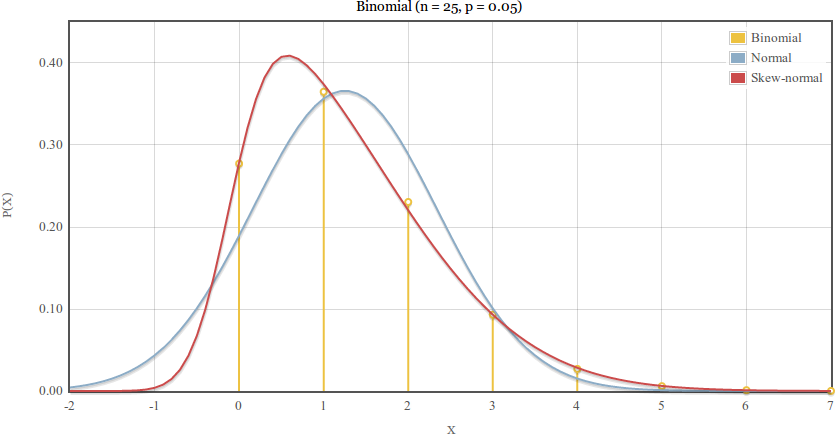
\includegraphics[width=\textwidth]{../images/binomial-normal-sn-2.png}}
    \only<3>{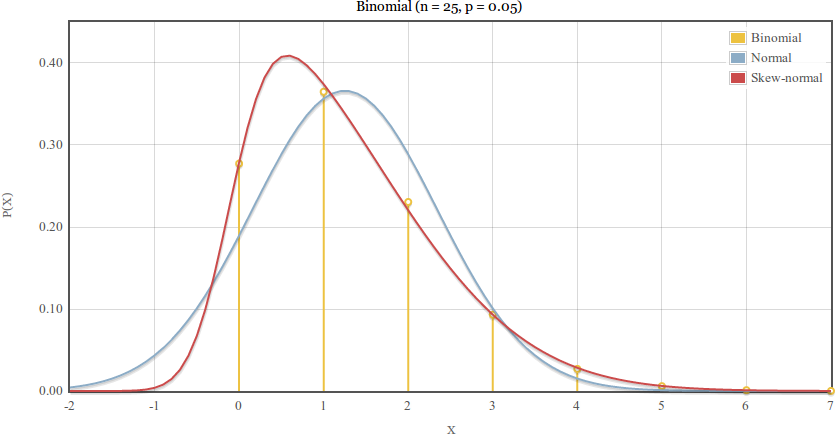
\includegraphics[width=\textwidth]{../images/binomial-normal-sn-3.png}}
  \end{center}
  \only<1>{the binomial is very skewed ...}
  \only<2>{and the normal approximation doesn't work very well.}
  \only<3>{Introducing ... the skew-normal distribution.}
}

%% Outline
\frame{ \frametitle{Outline}
  Today's itinerary:
  \begin{enumerate}[<+->]
    \item Skew-Normal distribution -- basic properties
    \item Method of Moments -- derive an approximation
    \item Accuracy -- examine the accuracy of our approximation
  \end{enumerate}
}
